During the implementation of the system, several problems were encountered. Each subsystem had its own set of problems, and the solutions to these problems are discussed below.

\subsubsection{Mechanical Design}
FDM printing or 3D printing is typically an iterative process, where the design is printed, tested, and then modified based on the results. This further reinforces the need for a modular and parametric design, as it allows for easy modification of each component. After a few iterations with errors due to tolerances and slightly incorrect measurements, (not relevant to the technical content of this report) a design was produced that physically fit together and mounted the components as intended, however when combined with the software and electronics, more problems were encountered that were eventually overcome by making some design decisions.

\begin{figure}[H]
    \centering
    \begin{minipage}[t]{0.49\textwidth}
        \centering
        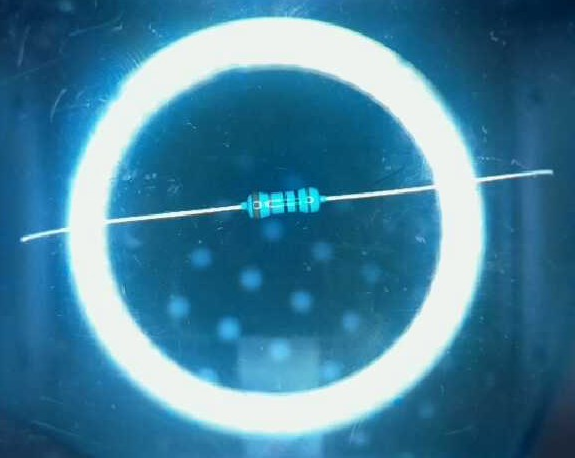
\includegraphics[height=6cm]{imgs/design/ringlight.jpg}
    \end{minipage}
    \hfill
    \begin{minipage}[t]{0.49\textwidth}
        \centering
        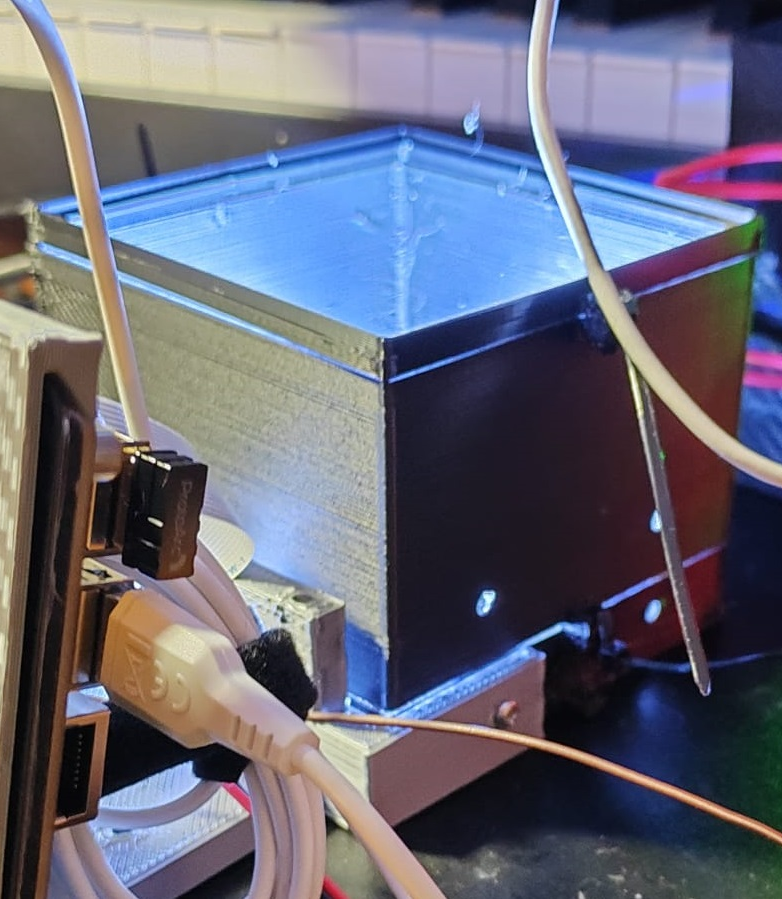
\includegraphics[height=6cm]{imgs/design/tallcamera.jpeg}
    \end{minipage}
    \caption{Glare from LED Ring and old camera housing}
    \label{fig:glare}
  \end{figure}

Originally, the system was to use a face-up camera with components mounted on an acrylic plate to allow the user to easily change the components as shown in \autoref{fig:glare}. However, this caused a problem with the LED ring, as the light would reflect off the acrylic plate, causing a glare that would obscure the image of the component. This design was then abandoned for the conveyor system that the system currently uses, as discussed in \autoref{sec:implementation-mechanical-design}.

\begin{figure}[H]
    \centering
    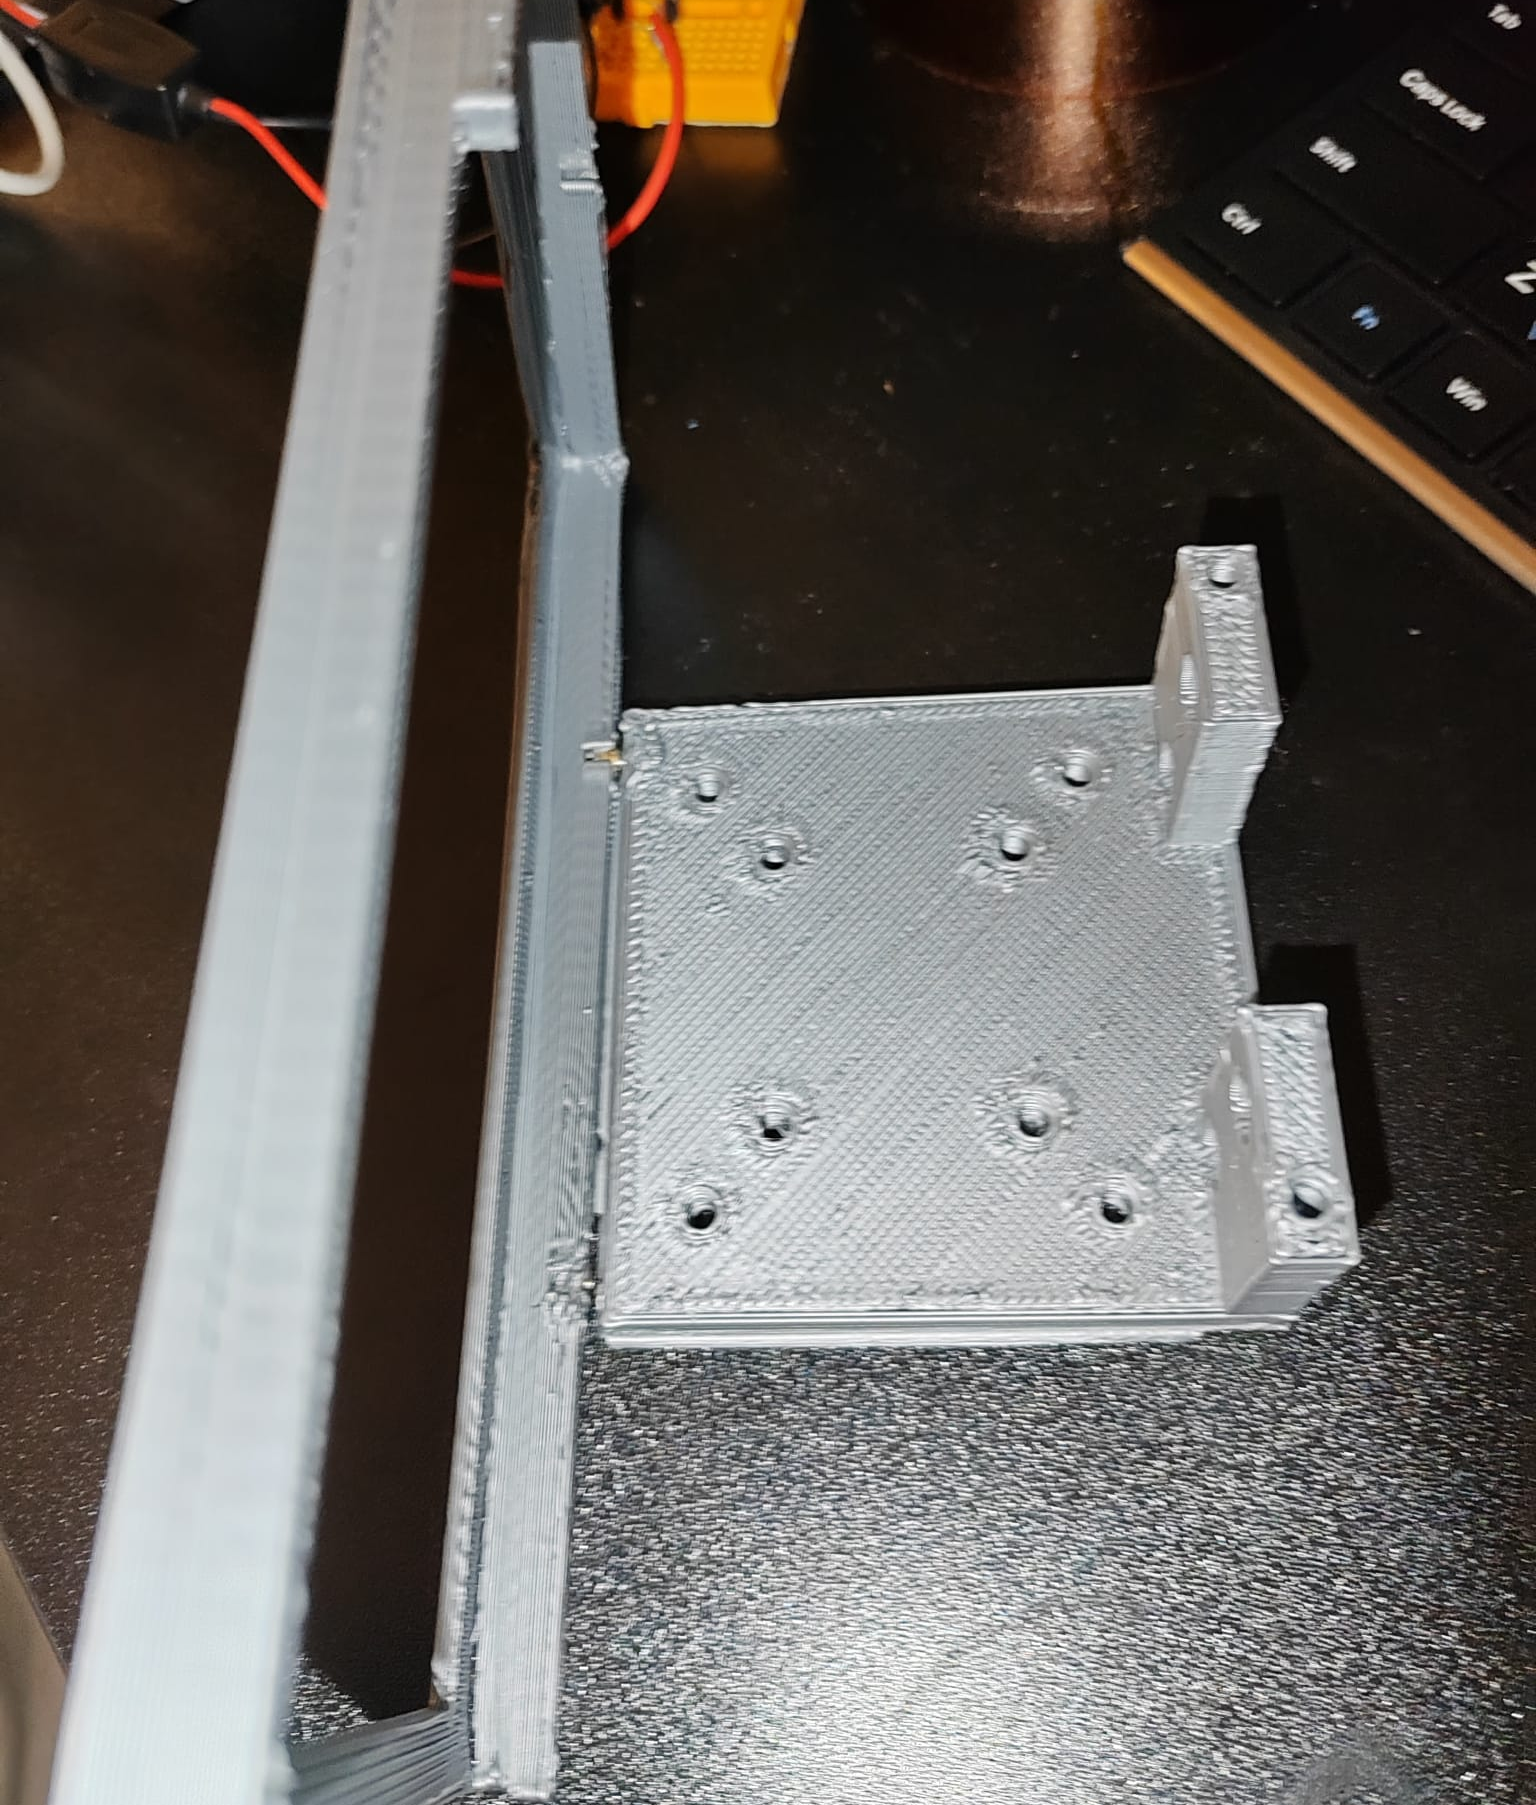
\includegraphics[height=8cm]{imgs/design/unbracedscreen.jpeg}
    \caption{Unbraced LCD Mount}
    \label{fig:brokenlcd}
  \end{figure}

 The initial design of the LCD cover was only mounted to the extrusion mount using two M3 screws at the base, which made it unstable and prone to wobbling. Over time, this would put stress on the plastic, causing it to break as shown in \autoref{fig:brokenlcd}. To solve this, a third mounting point was added to the LCD cover in the form of a brace that reaches halfway up the LCD cover, increasing the stability of the LCD, and preventing it from wobbling, as seen in \autoref{fig:lcdmount}.

 \begin{figure}[H]
    \centering
    \begin{minipage}[t]{0.49\textwidth}
        \centering
        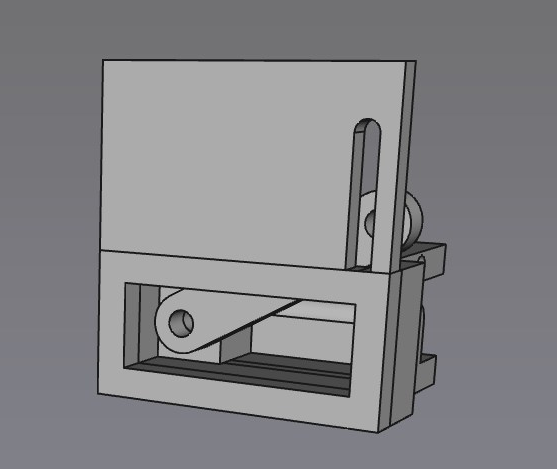
\includegraphics[height=6cm]{imgs/freecad/2024-05-14_22-32-02_FreeCADLink.jpg}
    \end{minipage}
    \hfill
    \begin{minipage}[t]{0.49\textwidth}
        \centering
        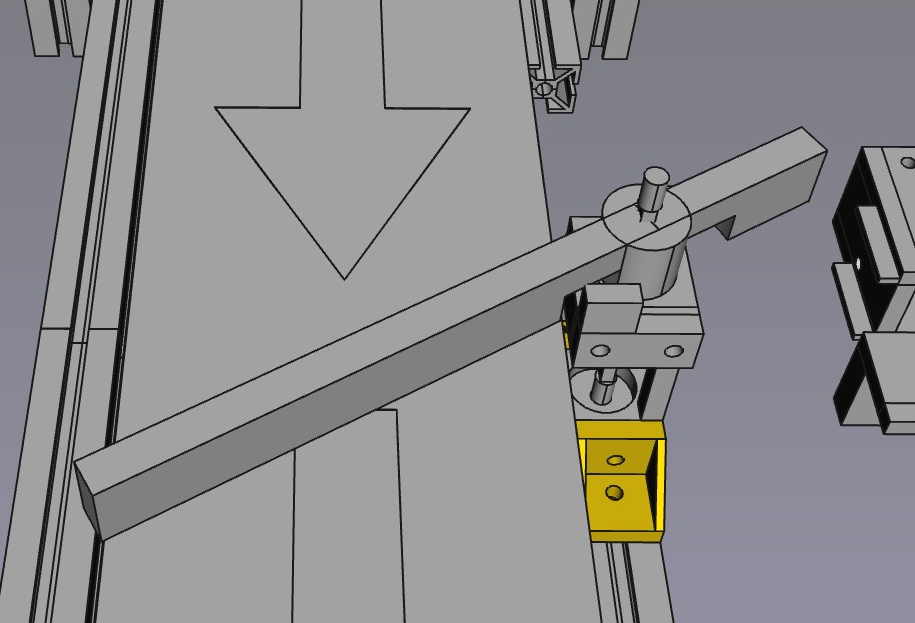
\includegraphics[height=6cm]{imgs/freecad/2024-05-13_17-56-29_FreeCADLink.jpg}
    \end{minipage}
    \caption{Linkage mechanism and old sweeper design}
    \label{fig:linkage}
  \end{figure}

 The bin sweeper also had several design iterations, however the main working principle was that the motor would drive a GT2 timing belt to move some other mechanism that would sweep the components, and this remained unchanged. The original design had several sweepers positioned at the bin locations, and would 'activate' like gates when the driven arm moved passed it. A flexible polyurethane rod was going to be used to allow the gates to be 'opened' by the arm, however the sweeper would then have to translate horizontal motion to vertical motion, which requires a complex mechanism using linkages as shown in \autoref{fig:linkage}. This was then simplified to a moving sweeper arm that was angled to use the conveyor belt speed to move the components off the belt, and was effective.
 
\subsubsection{Electronics and Wiring}
The WS2812B LED strip experienced communication issues when connected to the Raspberry Pi, often not responding to commands or flickering when attempting to do so. Originally, the strip was controlled via PWM (Pulse Width Modulation) however this requires root privileges and is not conventional. The solution was to use the SPI (Serial Peripheral Interface) protocol to control the strip, which does not require root privileges, however there was still flickering issues.

\begin{figure}[H]
    \centering
    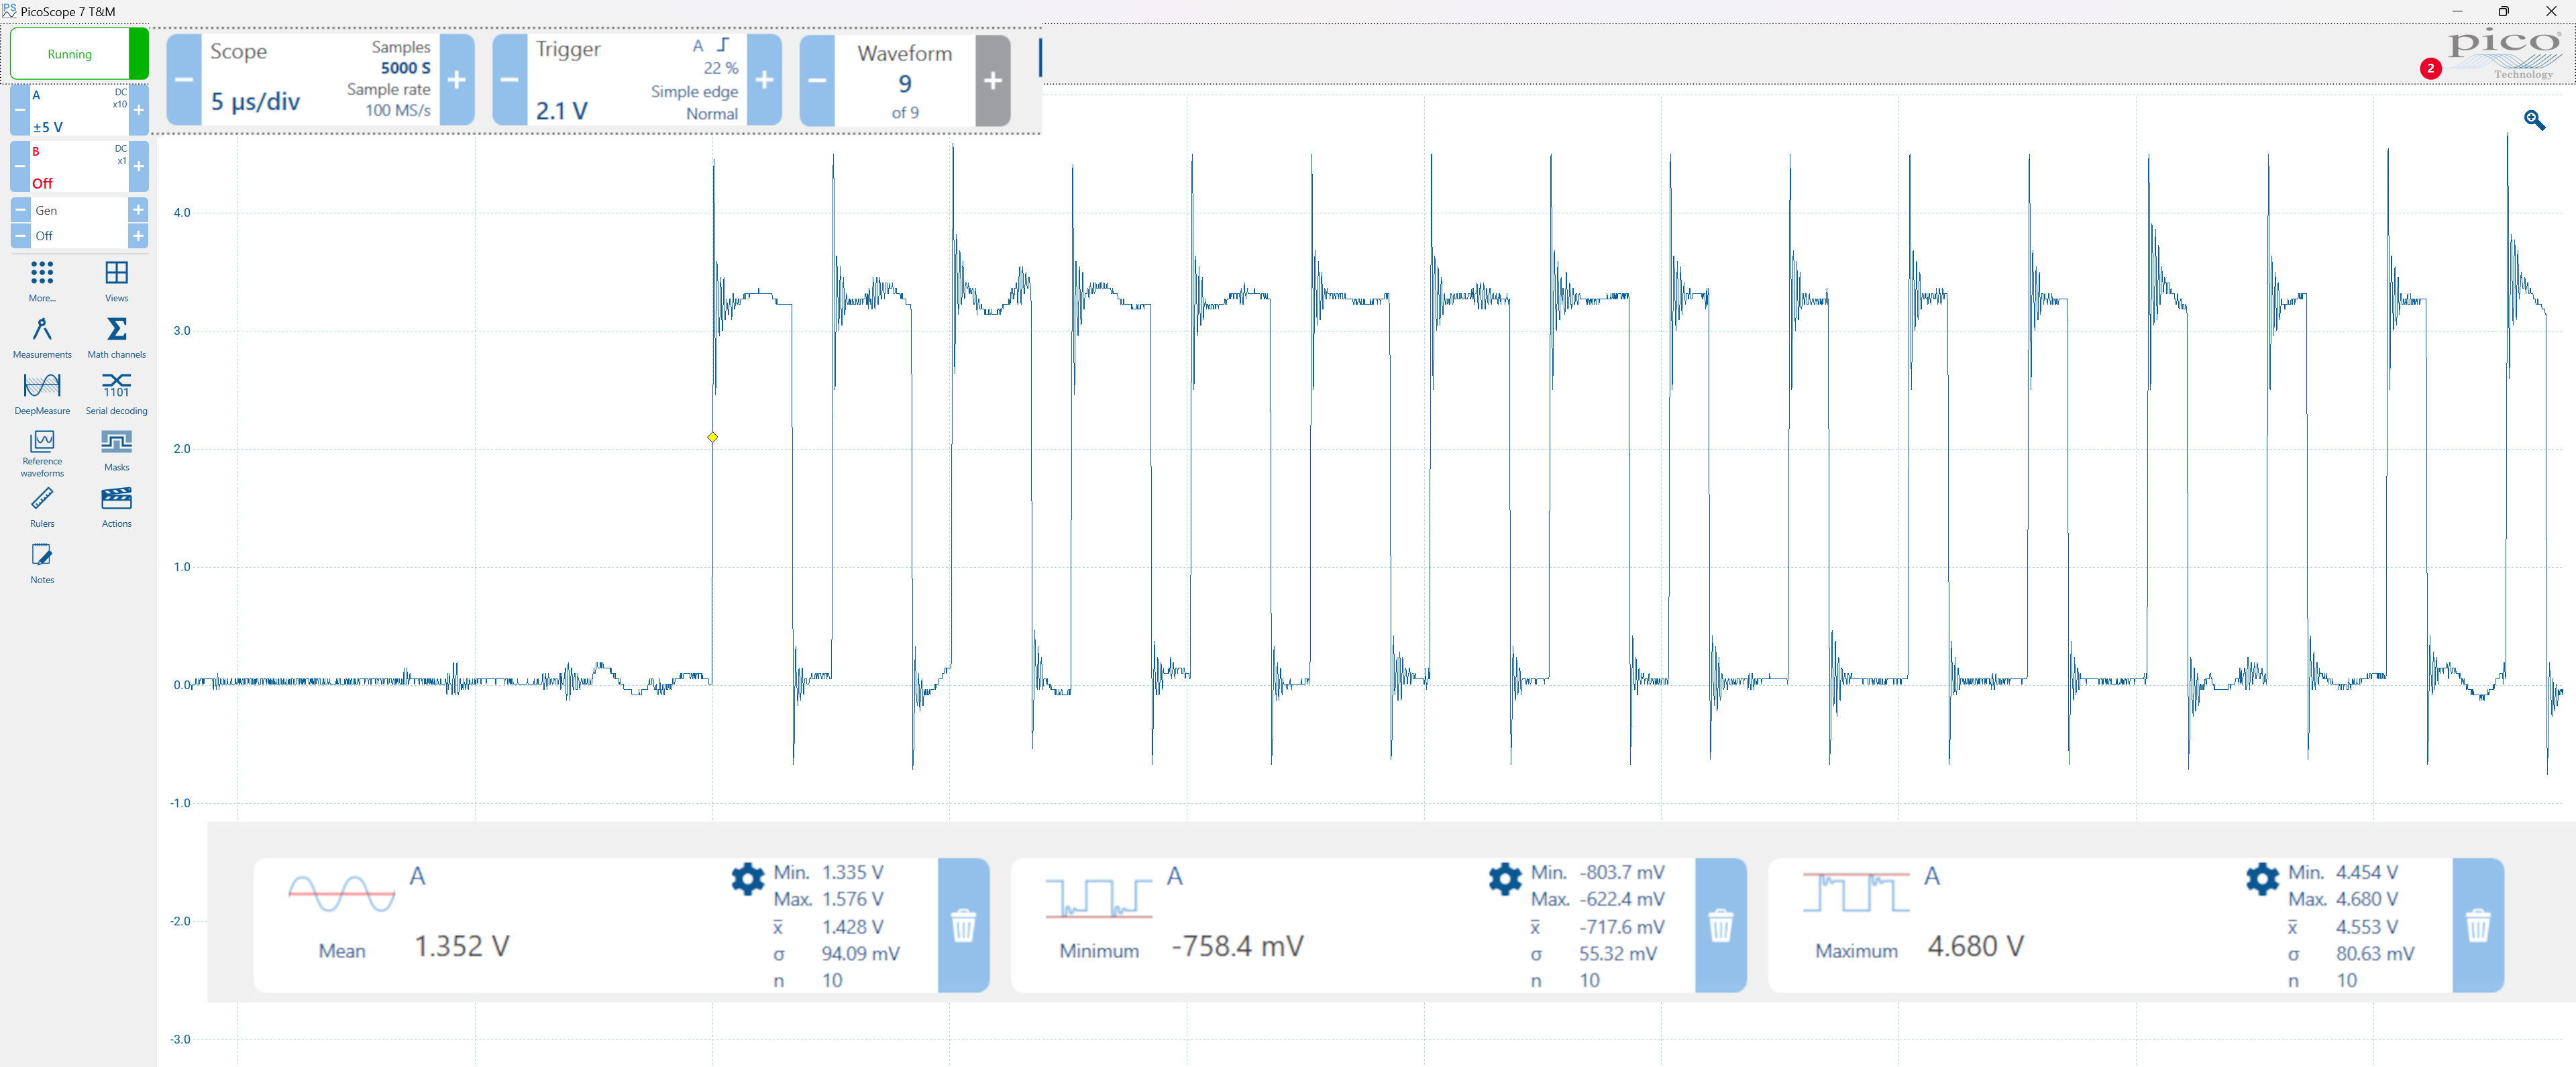
\includegraphics[width=\textwidth]{imgs/graphs/oscilloscope.png}
    \caption{PicoScope signal analysis}
    \label{fig:oscilloscope}
  \end{figure}

After several attempts to debug the issue programmatically, a PicoScope \cite{picoscope} was used to analyse the signal, and it was found that it was severely beneath the expected 5V signal, which was causing the flickering and general unresponsiveness of the strip. This can be seen in \autoref{fig:oscilloscope} (note the image has been edited to allow for better readability), with a maximum voltage of only 4.68V. The solution was to simply use thicker wires to connect the Raspberry Pi to the PSU, which solved the issue; despite the step-down converters display 5V, the voltage drop across the wires was causing the Pi to be undervolted, which was also shown on the display of the Pi itself in the corner as as lightning bolt symbol as shown in \autoref{fig:pi-undervolt}.
\begin{figure}[H]
    \centering
    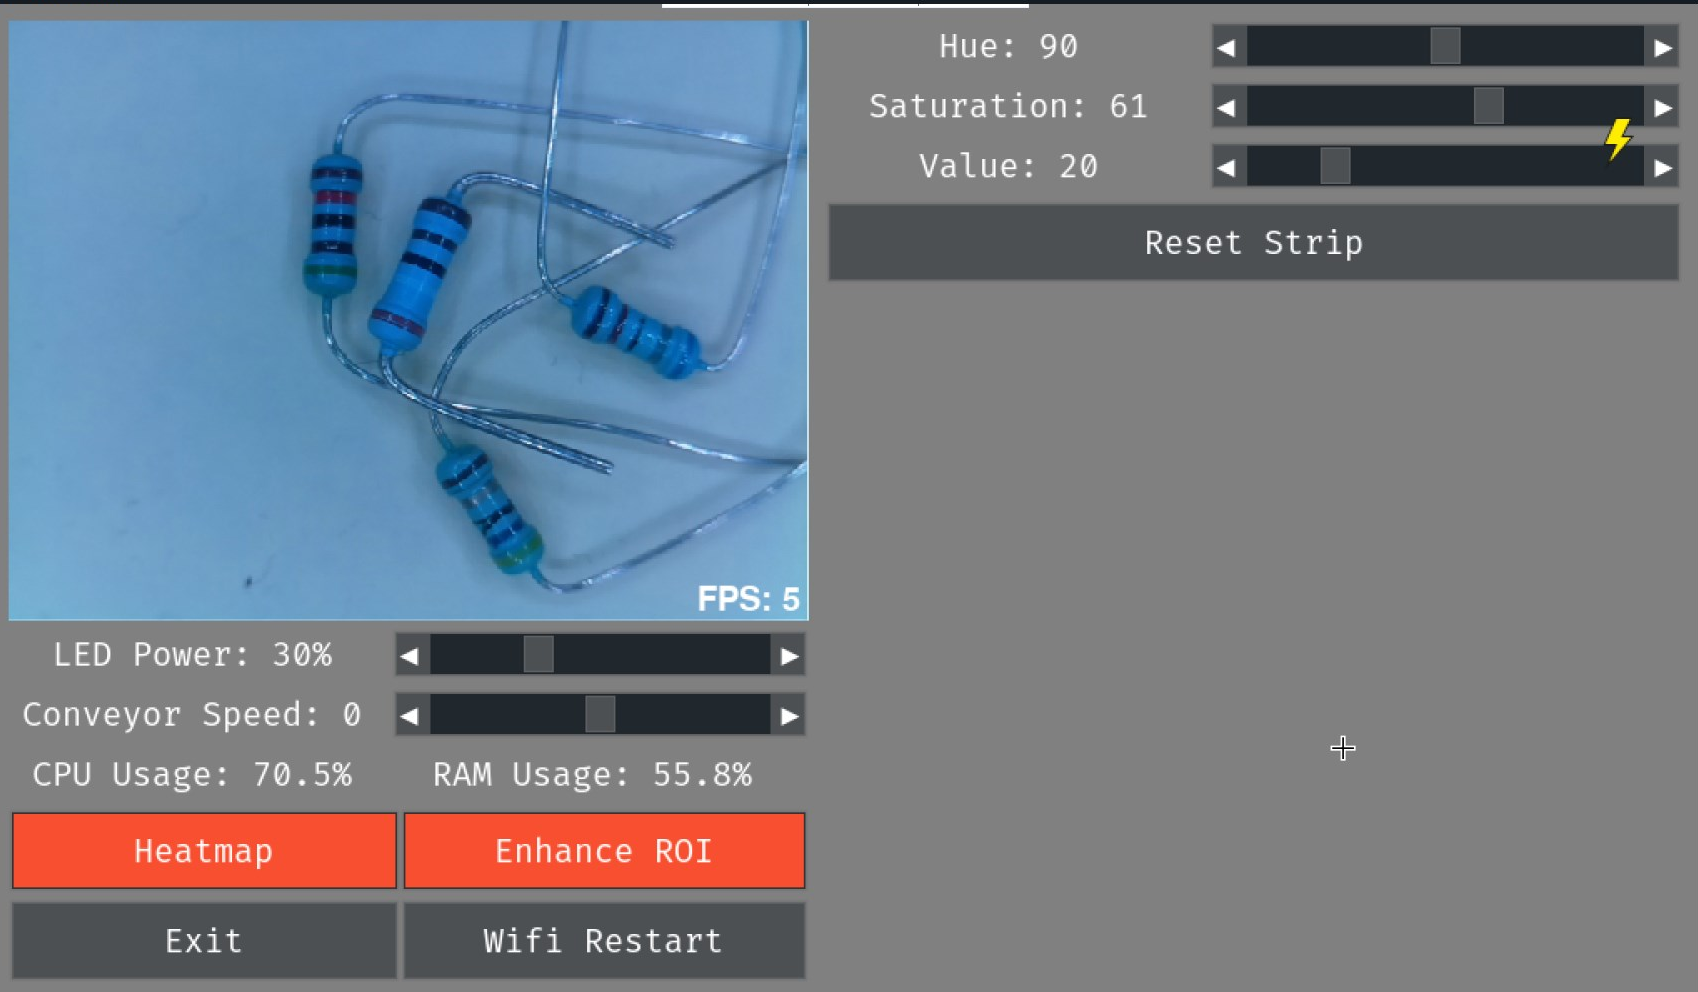
\includegraphics[height=8cm]{imgs/software/undervolt.jpg}
    \caption{Pi under-voltage warning}
    \label{fig:pi-undervolt}.
  \end{figure}

\subsubsection{Computer Vision}

\begin{figure}[H]
    \centering
    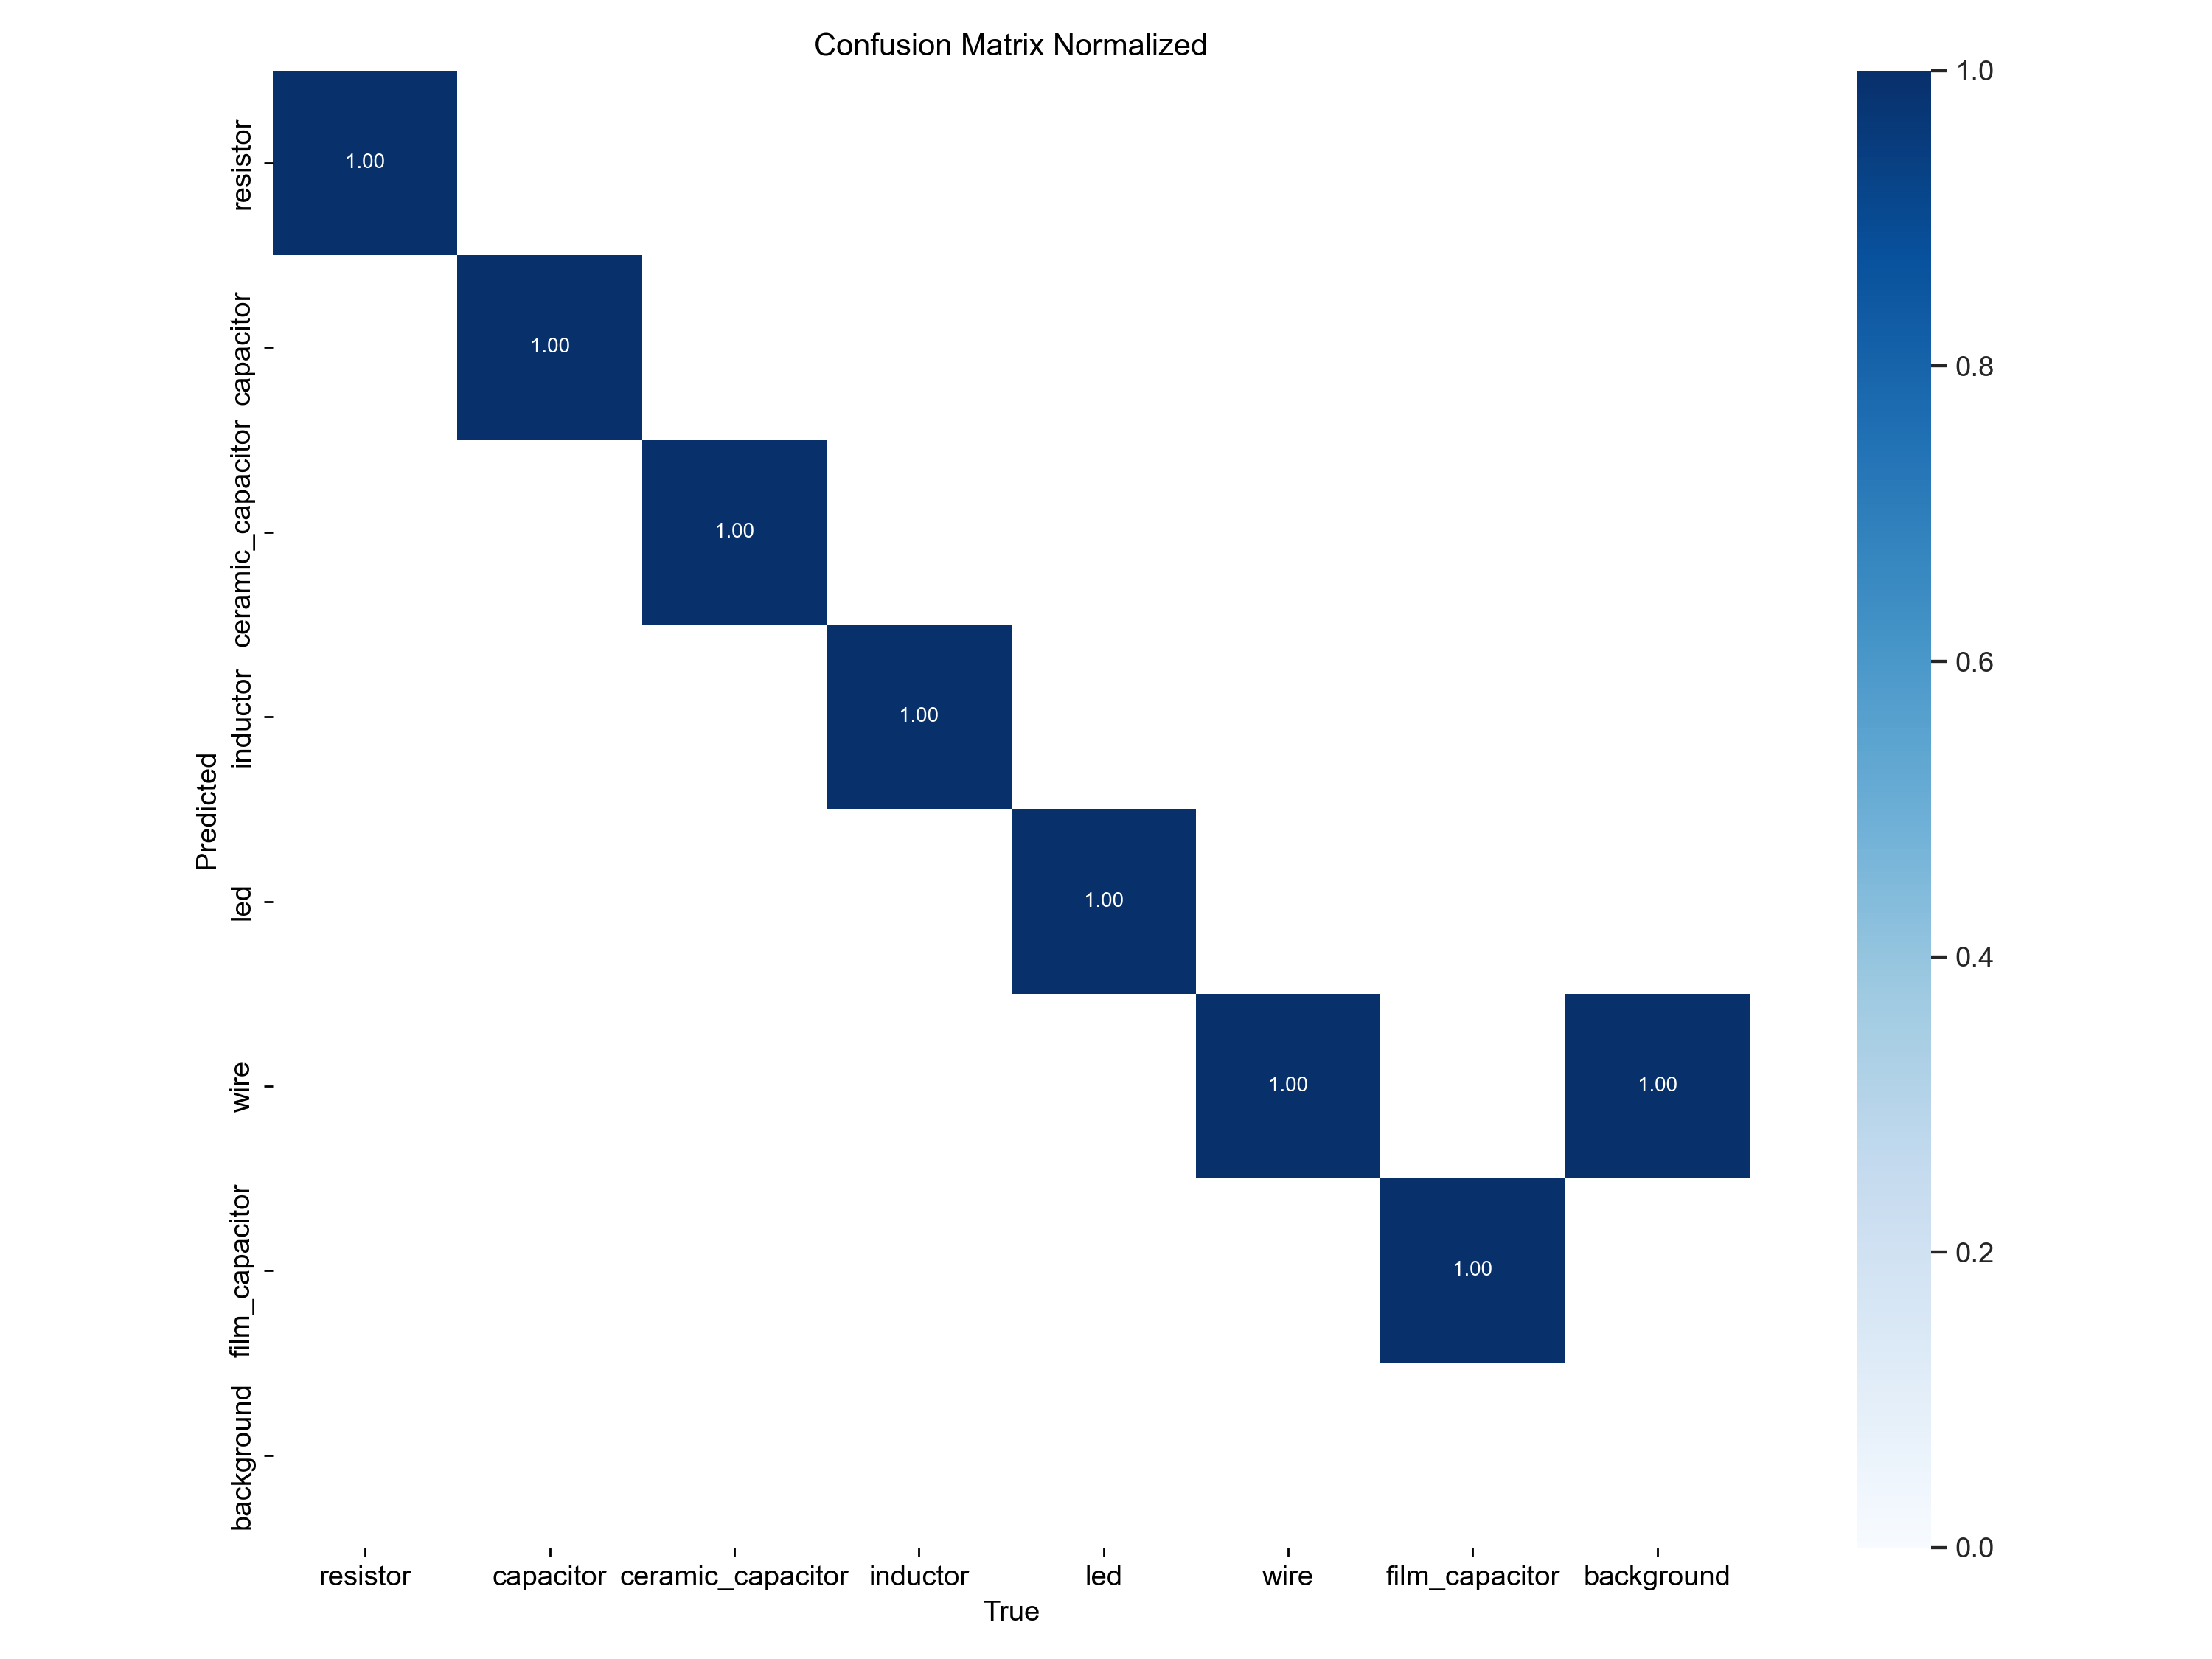
\includegraphics[width=0.8\textwidth]{imgs/graphs/confusion_matrix_test.png}
    \caption{Normalised confusion matrix for the test set}
    \label{fig:confusion-matrix}
  \end{figure}

During the evaluation of the model, the confusion matrix was examined to determine the model's performance on each class. The confusion matrix is shown in \autoref{fig:confusion-matrix}. Clearly, there is a strong diagonal line, which is a good sign as it shows that the model is correctly classifying most of the images, however interestingly there is a class that was unaccounted for during training; the background. 

Counterintuitively, the confusion matrix seems to imply that all background images are being classified as wires, but this is actually not what the confusion matrix is showing; it is showing that 100\% of false positives are wires, due to the fact that the confusion matrix is normalised. The unnormalised confusion matrix is shown in \autoref{fig:unconfusion-matrix}, where there are two false positives, and both are wires.

\begin{figure}[H]
    \centering
    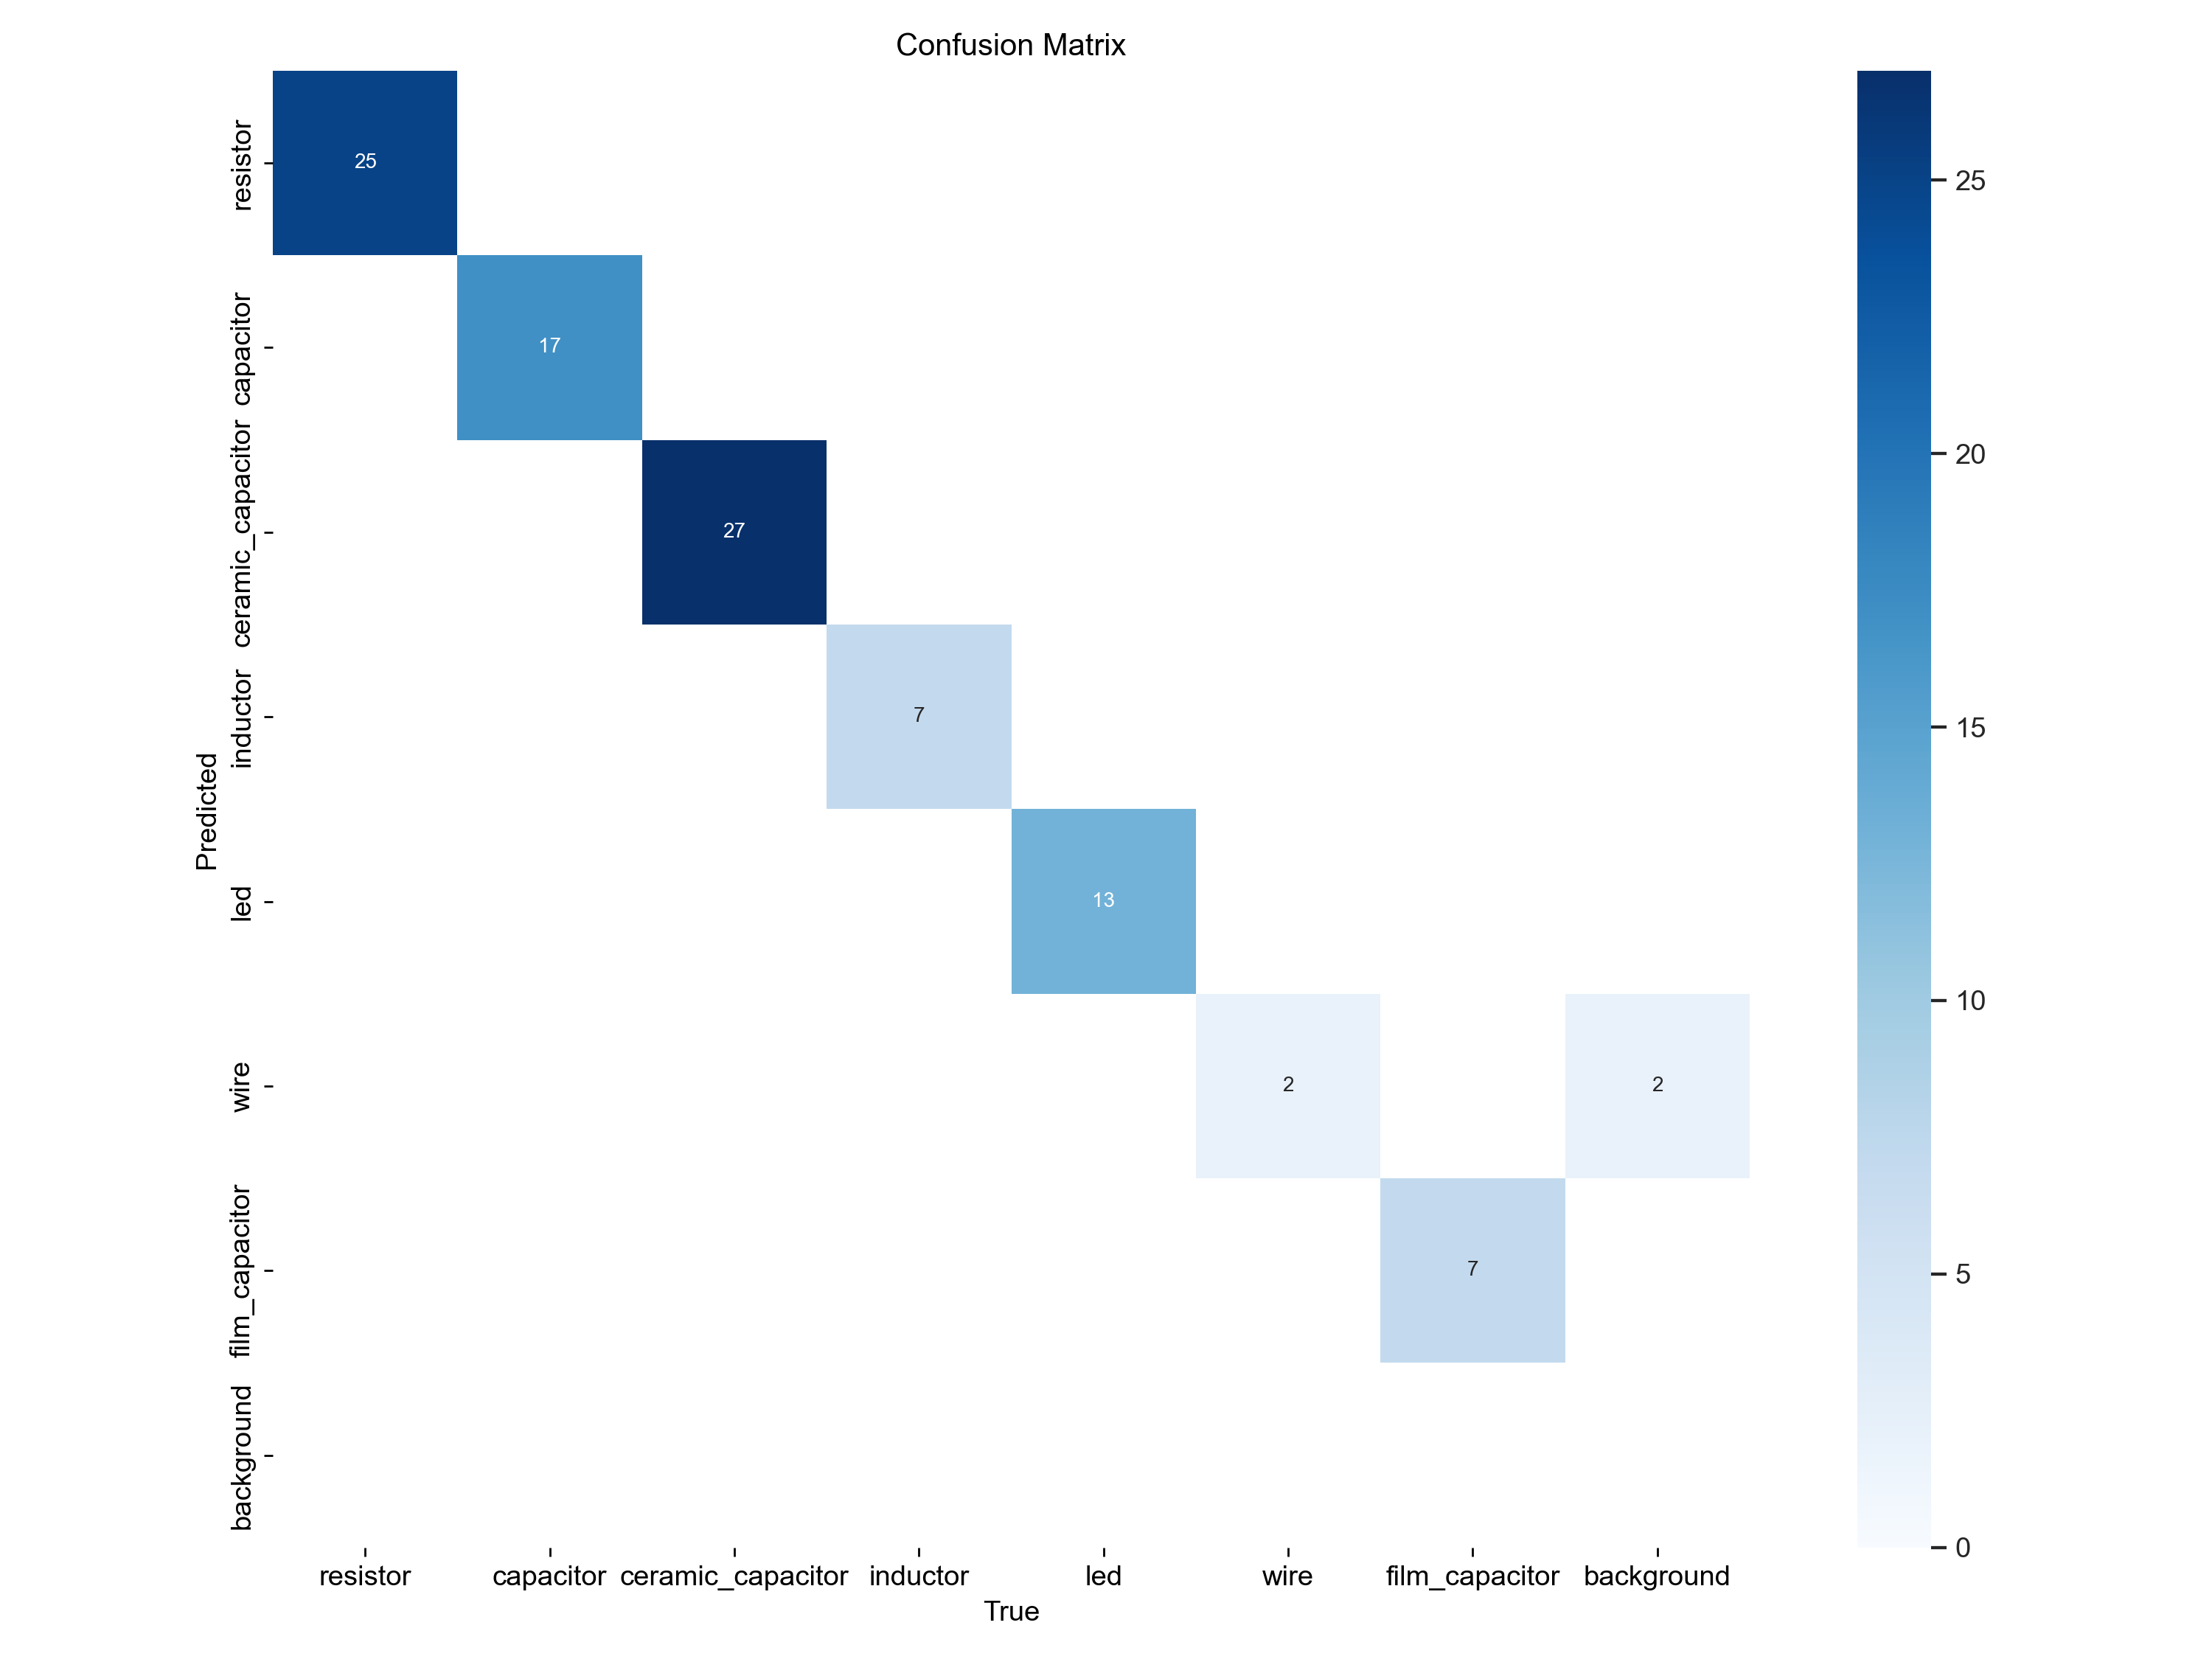
\includegraphics[width=0.8\textwidth]{imgs/graphs/unconfusion_matrix_test.png}
    \caption{Unnormalised confusion matrix for the test set}
    \label{fig:unconfusion-matrix}
  \end{figure}

However, this poses a problem; there are no images in the dataset without a component, so the model may have learnt that there is always a component in the image. This is a negative side effect of the dataset, as the model has not learnt that there are images without components, and thus will always place a bounding box, which is clearly not ideal. On Ultralytics' documentation \cite{ultralytics_2023} (the creators of YOLO), they state that "0-10\% background images to help reduce FPs" and that the COCO dataset "has 1000 background images for reference", which is 1\% of the total". Luckily, this was fixed extremely easily by adding images with no labels to the dataset, and the model will learn that there are images without components.

\begin{figure}[H]
    \centering
    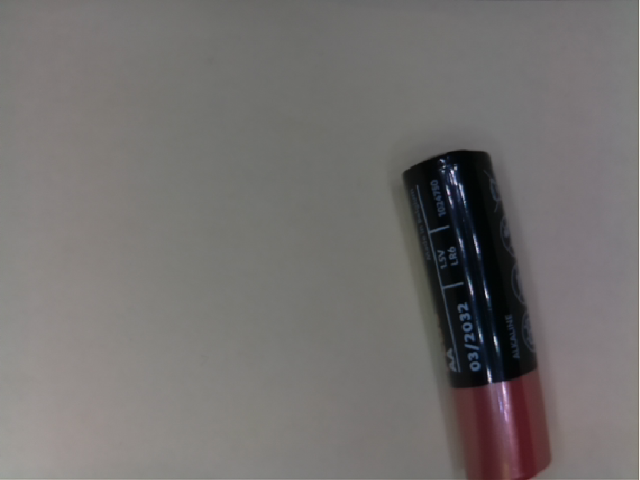
\includegraphics[width=0.8\textwidth]{imgs/cv/obb_background_1.png}
    \caption{Background image example}
    \label{fig:bg-image}
  \end{figure}
  
  As there are ~1000 images in the training set, 100 background images were added; however adding 100 images of the same static empty conveyor would not be very useful, so instead some images of the conveyor with a variety of objects were added to the dataset as shown in \autoref{fig:bg-image}, as well as other random images. The model was then retrained on this dataset, and the results are shown in. Naturally, the dataset annotation tool discussed in \label{sec:data-annotation-tool} was extended to allow for the addition of background images.
  
\begin{figure}[H]
    \centering
    \begin{minipage}[t]{0.49\textwidth}
        \centering
        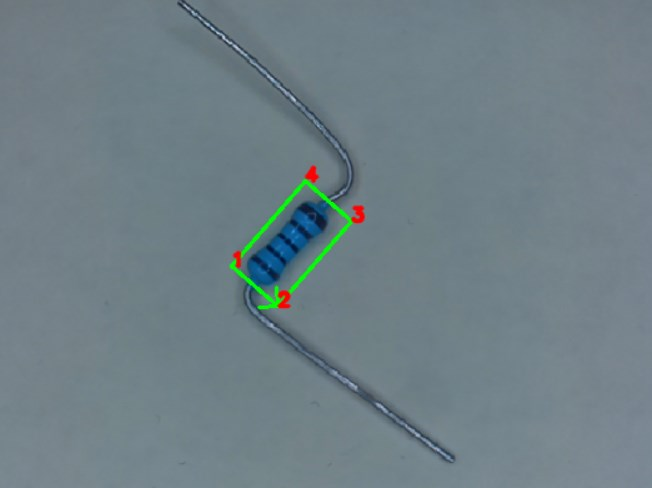
\includegraphics[height=6cm]{imgs/cv/numberedboundingbox.jpg}
    \end{minipage}
    \hfill
    \begin{minipage}[t]{0.49\textwidth}
        \centering
        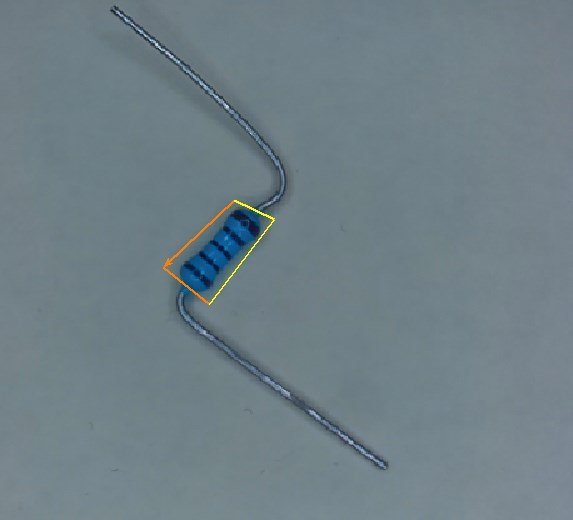
\includegraphics[height=6cm]{imgs/cv/resistor label.jpg}
    \end{minipage}
    \caption{Annotated resistor with orientation and vertex numbers on the same resistor during inference}
    \label{fig:obb-oritentation}
  \end{figure}

Also, it was discovered late into development that the OBB model does not learn the orientation of the components and encode it into the bounding box data. For instance, the line drawn between the first and second point does not indicate the orientation of the component, it is simply a line of the bounding box. This is shown more clearly in \autoref{fig:obb-oritentation}, where the resistor is annotated, with the first line drawn is an orange arrow to indicate the resistor's orientation, but during inference, the first line is a completely different line. At the time, this was an issue as to determine resistor values, it was necessary to know which way the resistor was facing to read the bands in the correct order. This was circumvented by adding a "stem" class for the resistor model to predict, where it would attempt to predict whether the first band of the resistor was. This is shown in \autoref{fig:resistorannotate} as the large yellow box that is drawn on the base of the resistor.